\begin{statementbox}
\textbf{\textcolor{CStatement}{一、条件与图形}}
\begin{description}[style=nextline,leftmargin=2.8em,labelsep=0.5em,itemsep=0.4em]
  \item[\textbf{条件一（横轴方向的抛物线）：}]
  抛物线 $y^2=2px$（$p\ne0$）上取两个\textbf{不同}的点
  $A(x_1,y_1)$、$B(x_2,y_2)$；过 $A,B$ 分别作切线，交于 $M$；弦 $AB$ 的中点为 $N$。
  \item[\textbf{条件二（纵轴方向的抛物线）：}]
  抛物线 $x^2=2py$（$p\ne0$）上的两个不同点同样记为 $A,B$，对应的切线交点、中点仍记为 $M,N$。
\end{description}

\par\noindent\begin{minipage}{\linewidth}
\begin{center}
\begingroup
\def\Cmode{0}
% Exact model: p=2, A=(1,-2), B=(4,4), M=(-2,1), N=(5/2,1).
\begin{tikzpicture}[x=1.15cm,y=0.85cm,>=stealth,font=\small]
\path[use as bounding box] (-3.1,-3.5) rectangle (6.1,5.2);
\draw[->,gray] (-2.9,0)--(5.7,0) node[right] {$x$};
\draw[->,gray] (0,-2.8)--(0,4.9) node[above] {$y$};
\node[below left] at (0,0) {$O$};
\draw[blue,thick,domain=-2.5:4.5,samples=100] plot ({\x*\x/4},\x);
\node[blue,right] at (5.1,4.2) {$y^2=4x$};
\draw[orange,thick] (-2.6,1.6)--(1.6,-2.6);
\draw[orange,thick] (-2.6,.7)--(5,4.5);
\draw[gray,thick] (1,-2)--(4,4);
\draw[red,very thick] (-2,1)--(2.5,1);
\ifnum\Cmode=1
  \draw[dashed,gray] (1,-2)--(-.55,-2) (4,4)--(-.55,4);
  \draw[<->,blue] (-.55,-2)--(-.55,1) node[midway,left,fill=white,inner sep=2pt] {$3$};
  \draw[<->,blue] (-.55,1)--(-.55,4) node[midway,left,fill=white,inner sep=2pt] {$3$};
  \fill[red] (0,1) circle (2pt) node[above left=2pt] {$H$};
\fi
\ifnum\Cmode=2
  \draw[dashed,blue] (1,-2)--(4,-2)--(4,4);
  \node[below,blue] at (2.5,-2.7) {$\Delta x=3$};
  \node[right,blue,fill=white,inner sep=2pt] at (4,-.6) {$\Delta y=6$};
  \node[fill=white,inner sep=3pt] at (2.8,4.85) {$AB:\ x=\tfrac12y+2,\quad pt=1$};
\fi
\ifnum\Cmode=3
  \node[fill=white,inner sep=3pt] at (2.7,4.85) {$AB:\ y=2(x-2)$};
  \node[anchor=west,fill=white,inner sep=3pt] at (3.4,2) {$y_1=-2,\ y_2=4$};
\fi
\ifnum\Cmode=4
  \draw[dashed,red] (-2,1)--(-2,-.7) (2.5,1)--(2.5,-.7);
  \draw[<->,red] (-2,-.6)--(2.5,-.6) node[pos=1,below right,fill=white,inner sep=3pt] {$x_N-x_M=\tfrac92>0$};
\fi
\fill (1,-2) circle (2pt) node[right=10pt] {$A(1,-2)$};
\fill (4,4) circle (2pt) node[above left] {$B(4,4)$};
\fill[red] (-2,1) circle (2pt) node[below left] {$M(-2,1)$};
\fill[red] (2.5,1) circle (2pt) node[below right,fill=white,inner sep=2pt] {$N(\tfrac52,1)$};
\ifnum\Cmode=0
  \node[red,above,fill=white,inner sep=3pt] at (.6,1) {$y_M=y_N=1$};
\fi
\end{tikzpicture}

\endgroup


图取 $p=2$：两切线（橙）交于 $M$，弦（灰）中点为 $N$；红色 $MN$ 水平。
\end{center}
\end{minipage}\par

\textbf{\textcolor{CStatement}{二、核心结论}}
\begin{description}[style=nextline,leftmargin=2.8em,labelsep=0.5em,itemsep=0.45em]
  \item[\textbf{结论一（$y^2=2px$）：}]
  切线交点与弦中点\textbf{纵坐标相同}：
  \[
    \boxed{y_M=y_N=\frac{y_1+y_2}{2}}.
  \]
  因为 $M\ne N$，直线 $MN$ 是水平直线：
  当 $y_1+y_2\ne0$ 时，$MN\parallel x$ 轴；
  当 $y_1+y_2=0$ 时，$MN$ \textbf{与 $x$ 轴重合}。
  \item[\textbf{结论二（$x^2=2py$）：}]
  切线交点与弦中点\textbf{横坐标相同}：
  \[
    \boxed{x_M=x_N=\frac{x_1+x_2}{2}}.
  \]
  直线 $MN$ 是竖直直线：当 $x_1+x_2\ne0$ 时，与 $y$ 轴平行；
  当 $x_1+x_2=0$ 时，\textbf{与 $y$ 轴重合}。
\end{description}

\par\noindent\begin{minipage}{\linewidth}
\begin{center}
\begin{tikzpicture}[x=1cm,y=1cm,>=stealth,font=\small]
\path[use as bounding box] (-3,-2.5) rectangle (5.1,4.6);
\draw[->,gray] (-2.8,0)--(4.8,0) node[right] {$x$};
\draw[->,gray] (0,-2.2)--(0,4.2) node[above] {$y$};
\node[below left] at (0,0) {$O$};
\draw[blue,thick,domain=-2.5:4,samples=90] plot (\x,{\x*\x/4});
\node[blue,right] at (3.8,3.5) {$x^2=4y$};
\draw[orange,thick] (-2.4,1.4)--(1.4,-2.4) (.8,-2.4)--(4,4);
\draw[gray,thick] (-2,1)--(4,4);
\draw[red,very thick] (1,-2)--(1,2.5);
\fill (-2,1) circle (2pt) node[below left=3pt] {$A(-2,1)$};
\fill (4,4) circle (2pt) node[above left] {$B(4,4)$};
\fill[red] (1,-2) circle (2pt) node[right] {$M(1,-2)$};
\fill[red] (1,2.5) circle (2pt) node[above left] {$N(1,\tfrac52)$};
\node[red,right,fill=white,inner sep=3pt] at (1,.7) {$x_M=x_N=1$};
\end{tikzpicture}


交换横、纵坐标后，红色 $MN$ 变为竖直方向。
\end{center}
\end{minipage}\par

\textbf{\textcolor{CStatement}{三、进一步的精确坐标（便于验算和做题）}}
对于 $y^2=2px$，还有
\[
\boxed{M\left(\frac{y_1y_2}{2p},\frac{y_1+y_2}{2}\right),\quad
N\left(\frac{y_1^2+y_2^2}{4p},\frac{y_1+y_2}{2}\right).}
\]
\[
\boxed{x_N-x_M=\frac{(y_1-y_2)^2}{4p}\ne0,\qquad
|MN|=\frac{(y_1-y_2)^2}{4|p|}>0.}
\]
当 $p>0$ 时，$N$ 在 $M$ 右侧；当 $p<0$ 时，$N$ 在 $M$ 左侧。

\medskip
\textbf{\textcolor{CStatement}{使用提醒}}
两个切点可以在对称轴的两侧，也可以有一个是顶点；不需要假定切点处切线的斜率存在。
\end{statementbox}
